\documentclass[conference]{IEEEtran}
\IEEEoverridecommandlockouts
\usepackage{cite}
\usepackage{amsmath,amssymb,amsfonts}
\usepackage{algorithmic}
\usepackage{graphicx}
\usepackage{textcomp}
\usepackage{xcolor}
\usepackage[italian]{babel}

\begin{document}

\title{Canny Edge Detector: studio e implementazione}

\author{\IEEEauthorblockN{Martin Trajkovski}
\IEEEauthorblockA{\textit{Corso di Laurea in Scienze Informatiche} \\
\textit{Universit\`a degli Studi di Parma}\\
Matricola: 397464}
}

\maketitle

\begin{abstract}
Studio e implementazione da zero in NumPy del Canny Edge Detector. La pipeline
copre smoothing gaussiano, gradiente con filtri di Sobel, non-maximum
suppression, double threshold e hysteresis, secondo il programma del corso
(filtri lineari, derivate parziali, convoluzione 2D).
\end{abstract}

\section{Introduzione}
L'\textit{edge detection} mira a estrarre i contorni di un'immagine come luoghi
di forte variazione di luminanza. Il rilevatore di Canny~\cite{canny1986}
combina filtraggio, derivazione e sogliatura in una pipeline robusta e ancora
oggi standard di riferimento.

\section{Pipeline}
Sia $I:\mathbb{R}^2\to\mathbb{R}$ l'immagine in scala di grigi. La pipeline
applicata \`e:

\textbf{1. Smoothing.} Convoluzione con kernel gaussiano
$G_\sigma(x,y)=\frac{1}{2\pi\sigma^2}\exp\!\left(-\frac{x^2+y^2}{2\sigma^2}\right)$
per ridurre il rumore: $I_s = I * G_\sigma$.

\textbf{2. Gradiente.} Approssimazione discreta tramite filtri di Sobel:
$G_x = I_s * S_x,\ G_y = I_s * S_y$, da cui magnitudo
$M=\sqrt{G_x^2+G_y^2}$ e direzione $\theta=\arctan2(G_y,G_x)$.

\textbf{3. Non-Maximum Suppression.} Per ogni pixel si discretizza $\theta$ in
uno dei quattro settori $\{0^\circ,45^\circ,90^\circ,135^\circ\}$ e si conserva
$M(i,j)$ solo se massimo locale lungo la direzione del gradiente.

\textbf{4. Double Threshold.} Definite due soglie $T_l<T_h$ relative a
$\max M$, i pixel sono classificati come \emph{forti} ($\ge T_h$),
\emph{deboli} ($T_l\le \cdot < T_h$) o scartati.

\textbf{5. Hysteresis.} I pixel deboli vengono promossi a edge se connessi
(8-vicinato) a un pixel forte; gli altri sono soppressi.

\section{Risultati}
L'algoritmo \`e stato testato su immagini reali con $\sigma=1.4$,
kernel $5\times 5$, $T_l=0.05\cdot\max M$, $T_h=0.15\cdot\max M$.
La Figura~\ref{fig:pipeline} mostra gli stadi intermedi della pipeline.

\begin{figure}[h]
\centering

\includegraphics[width=\columnwidth]{pipeline.png}
\caption{Stadi della pipeline: grayscale, smoothing, magnitudo del gradiente,
NMS, double threshold, edge finali.}
\label{fig:pipeline}
\end{figure}

\begin{figure}[h]
\centering
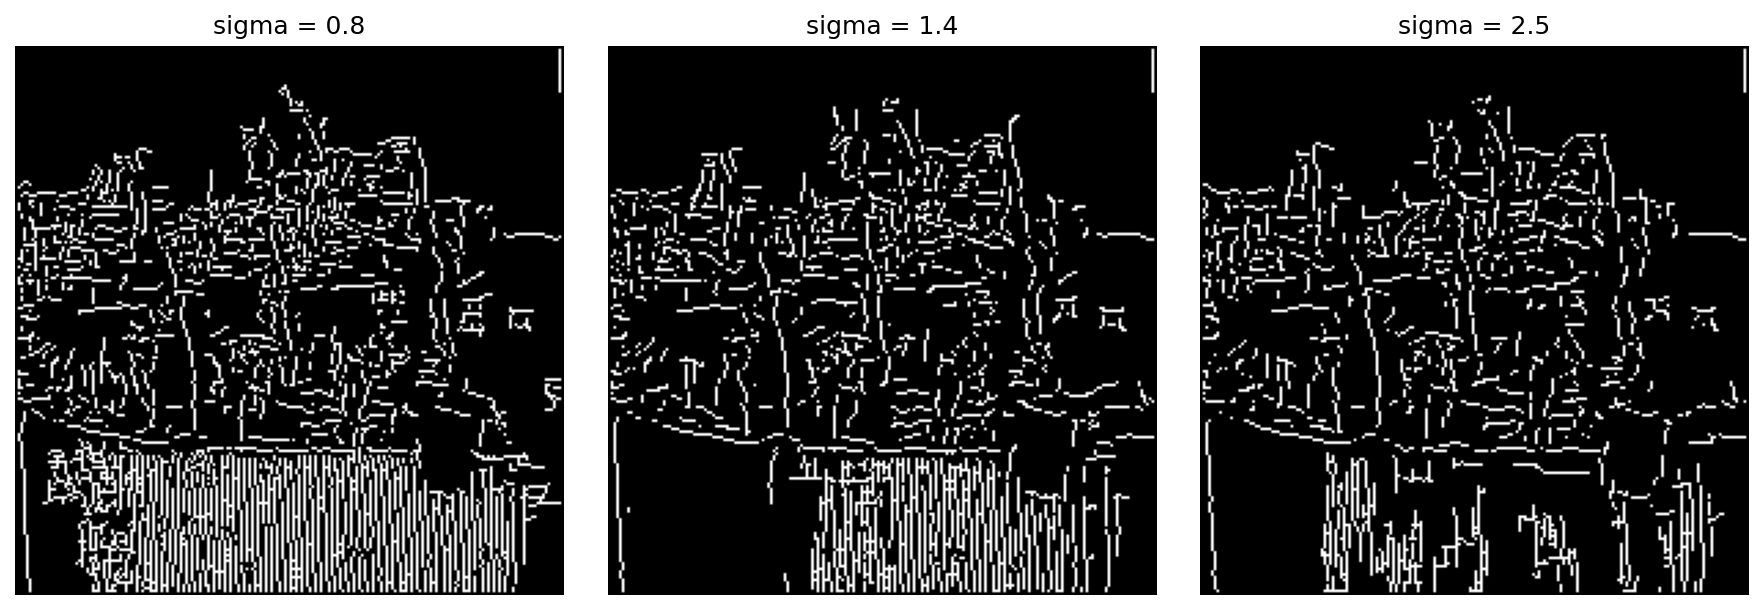
\includegraphics[width=\columnwidth]{sigma_comparison.png}
\caption{Effetto di $\sigma$: a $\sigma=0.8$ emergono molti dettagli ma anche
rumore tessiturale; a $\sigma=2.5$ i bordi sono pi\`u puliti ma meno localizzati.}
\label{fig:sigma}
\end{figure}

\section{Conclusioni}
L'implementazione conferma che le quattro idee chiave del corso --- convoluzione
2D, derivate via Sobel, sogliatura adattiva e connessione di componenti ---
bastano a costruire un rilevatore di bordi competitivo. Il parametro pi\`u
critico \`e $\sigma$: valori bassi preservano i dettagli ma amplificano il
rumore, valori alti producono bordi pi\`u puliti ma meno localizzati.

\begin{thebibliography}{1}
\bibitem{canny1986} J. Canny, ``A Computational Approach to Edge Detection,''
\textit{IEEE Trans. Pattern Anal. Mach. Intell.}, vol. PAMI-8, no. 6, 1986.
\end{thebibliography}

\end{document}
